\begin{frame}
  \frametitle{\texttt{pgfplots}}

\end{frame}

\begin{frame}
  \frametitle{Functies plotten}

  \begin{columns}
    \begin{column}{.4\textwidth}
      \inputminted[fontsize = \scriptsize]{latex}{tikz/pgfplots/parabola.tikz}
    \end{column}
    \begin{column}{.6\textwidth}
      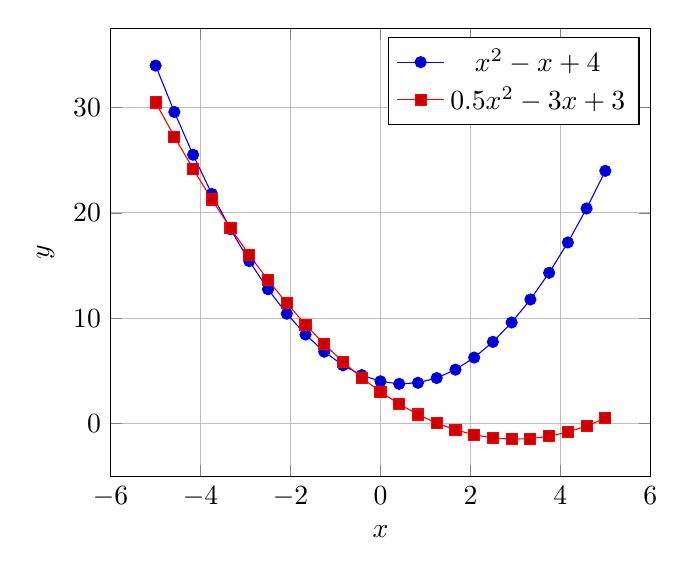
\begin{tikzpicture}
  \begin{axis}[
    grid=major,
    xlabel=$x$,
    ylabel=$y$
  ]
    \addplot {x^2 - x + 4};
    \addlegendentry{$x^2-x+4$};
    \addplot {.5*x^2 - 3*x + 3};
    \addlegendentry{$0.5x^2-3x+3$};
  \end{axis}
\end{tikzpicture}

    \end{column}
  \end{columns}
\end{frame}

\begin{frame}
  \frametitle{Datasets plotten}

  \begin{columns}
    \begin{column}{.4\textwidth}
      \inputminted[fontsize = \scriptsize]{latex}{tikz/pgfplots/external.tikz}
    \end{column}
    \begin{column}{.6\textwidth}
      \begin{tikzpicture}
  \begin{axis}[
    grid=major,
    xlabel=$x$,
    ylabel=$y$
  ]
    \addplot table[x = x, y = f]
      {tikz/pgfplots/data.dat};
    \addlegendentry{$x^2-x+4$};
    \addplot table[x = x, y = g]
      {tikz/pgfplots/data.dat};
    \addlegendentry{$0.5x^2-3x+3$};
  \end{axis}
\end{tikzpicture}

    \end{column}
  \end{columns}
\end{frame}

\begin{frame}
  \frametitle{De dataset}

  \inputminted[lastline = 10]{latex}{tikz/pgfplots/data.dat}
\end{frame}

\begin{frame}
  \frametitle{Contour plots}

  \centering
  \begin{tikzpicture}[scale = .5]
  \begin{axis}[
    colormap name=whitered,
    3d box,
    width=15cm,
    view={25}{25},
    enlargelimits=false,
    grid=major,
    domain=-0.5:4.7,
    y domain=-2:2,
    samples=21,
    xlabel=$x$,
    ylabel=$\dot{x}$,
    zlabel={$\text{E}_{\text{m}}$},
    colorbar,
    colorbar style={
        at={(1,0)},
        anchor=south west,
        height=0.1*\pgfkeysvalueof{/pgfplots/parent axis height},
        title={$\text{E}_{\text{m}}(x,\dot{x})$}
        },
    colormap={whitered}{color(0cm)=(white); color(1cm)=(orange!75!red)}
    ]
    \addplot3 [y domain = 0:2, surf]
      {-0.7+4*exp(-0.5*(x+3))*(3*cos(4*x*180/pi)+2.5*cos(2*x*180/pi))
       + 0.5*y*y*4};

    \addplot3 [y domain = 0:2, contour gnuplot = {number=14, labels={false},
      draw color = ugentblue}, samples = 21, ]
      {-0.7+4*exp(-0.5*(x+3))*(3*cos(4*x*180/pi)+2.5*cos(2*x*180/pi))
       + 0.5*y*y*4};

    \addplot3 [domain = -0.5:4.7, samples = 31, samples y = 0, thick, smooth]
        (x,-2,{-0.6+4*exp(-0.5*(x+3))*(3*cos(4*x*180/pi)+2.5*cos(2*x*180/pi))});
    \addplot3 [contour gnuplot = {number=14, labels={false}, draw color=ugentblue},
        samples=21,z filter/.code={\def\pgfmathresult{20}}]
        {-0.7+4*exp(-0.5*(x+3))*(3*cos(4*x*180/pi)+2.5*cos(2*x*180/pi))
         + 0.5*y*y*4};
    \addplot3 [y domain=-2:0,surf]
        {-0.7+4*exp(-0.5*(x+3))*(3*cos(4*x*180/pi)+2.5*cos(2*x*180/pi))
         + 0.5*y*y*4};
    \addplot3 [domain = 0:.25, contour gnuplot = {number=14,labels={false},
        draw color=ugentblue}, samples=21]
        {-0.7+4*exp(-0.5*(x+3))*(3*cos(4*x*180/pi)+2.5*cos(2*x*180/pi))
         + 0.5*y*y*4};
  \end{axis}
\end{tikzpicture}


  \small\url{http://pgfplots.net/tikz/examples/contour-surface/}
\end{frame}

\begin{frame}
  \frametitle{Weierstrassfunctie}

  \centering
  \begin{luacode}
  function weierstrass(x0, x1, n, a, b, epsilon)
    local dx = (x1-x0)/n 
    local x = x0
    local out=assert(io.open("tmp.data","w"))
    local y,k,dy
    while (x <= x1) do
      y = 0
      k = 0
      repeat
        dy = math.pow(a,k) * math.cos(math.pow(b,k)*math.pi*x)
        y = y + dy
        k = k + 1
      until (math.abs(dy) < epsilon)
      out:write(x, " ", y, "\string\n") 
      x = x + dx
    end
    out:close()
  end
\end{luacode}

\begin{tikzpicture}[every pin/.style={fill=white},pin distance=1.2cm]
  \directlua{weierstrass(-2,2,5000,0.3,5,1.e-12)}%
  \begin{axis}[axis lines=middle,domain=-2:2]
    \addplot [thin, line join=round] table {tmp.data};
    \coordinate (p1) at (axis cs:1,-1.38);
    \coordinate (p2) at (axis cs:1.8,0.6);
    \coordinate (legend) at (axis cs:0,2);
  \end{axis}
  \directlua{weierstrass(0.95,1.05,5000,0.3,5,1.e-12)}%
  \node[pin=3:{%
    \begin{tikzpicture}[baseline,trim axis left,trim axis right]
      \begin{axis}[tiny,axis lines=box,domain=0.95:1.05,scale=0.5]
        \addplot [thin, line join=round] table {tmp.data};
      \end{axis}
    \end{tikzpicture}%
  }] at (p1) {};
  \directlua{weierstrass(1.7,1.9,5000,0.3,5,1.e-12)}%
  \node[pin=3:{%
    \begin{tikzpicture}[baseline,trim axis left,trim axis right]
      \begin{axis}[tiny,axis lines=box,domain=1.7:1.9]
        \addplot [thin, line join=round] table {tmp.data};
      \end{axis}
    \end{tikzpicture}%
  }] at (p2) {};
  \node at (legend)
    {$\displaystyle f(x) = \sum_{n=0}^\infty a^n \cos(b^n \pi x)$};
\end{tikzpicture}


  \small\url{http:/pgfplots.net/tikz/examples/weierstrass-function/}
\end{frame}

